\documentclass[10pt]{beamer}

\usetheme{Madrid}
\usecolortheme{default}
\usefonttheme{serif}
\setbeamertemplate{navigation symbols}{}

% --- PACKAGES ---
\usepackage[utf8]{inputenc}
\usepackage[T1]{fontenc}
\usepackage{graphicx}
\usepackage{amsmath}
\usepackage{amsfonts}
\usepackage{amssymb}
\usepackage{booktabs}
\usepackage{tabularx}
\usepackage{listings}
\usepackage{xcolor}

% --- LISTINGS (CODE) SETUP ---
\definecolor{codegreen}{rgb}{0,0.6,0}
\definecolor{codegray}{rgb}{0.5,0.5,0.5}
\definecolor{codepurple}{rgb}{0.58,0,0.82}
\definecolor{backcolour}{rgb}{0.95,0.95,0.92}

\lstdefinestyle{mystyle}{
    backgroundcolor=\color{backcolour},
    commentstyle=\color{codegreen},
    keywordstyle=\color{magenta},
    numberstyle=\tiny\color{codegray},
    stringstyle=\color{codepurple},
    basicstyle=\ttfamily\footnotesize, % Using footnotesize for code now
    breakatwhitespace=false,
    breaklines=true,
    captionpos=b,
    keepspaces=true,
    numbers=left,
    numbersep=5pt,
    showspaces=false,
    showstringspaces=false,
    showtabs=false,
    tabsize=2,
    frame=tb,
    xleftmargin=1em % Add some left margin to code blocks
}
\lstset{style=mystyle}

% --- TITLE PAGE INFORMATION ---
\title[IntelliGaze]{
\includegraphics[height=1.5cm]{images/bgc-logo.png}\\[1em] IntelliGaze: A Wearable AI Camera System}
\subtitle{Microprocessor Lab Project Presentation}
\author[Team Rustacean]{
    Touhidul Alam Seyam (230240003) \and
    Eftakar Uddin (230240004) \and
    Tasmim Akther Mim (230240025) \and
    Shafiul Azam Mahin (230240022) \and
    Muntasir Rahman (230240002)
}
\institute[BGC Trust University]{
    Department of Computer Science and Engineering \\
    BGC Trust University Bangladesh
}
\date{June 16, 2025}

% --- DOCUMENT START ---
\begin{document}

% --- TITLE SLIDE ---
\begin{frame}
    \titlepage
\end{frame}

% --- OUTLINE SLIDE ---
\begin{frame}{Outline}
    \tableofcontents
\end{frame}

% --- SECTION: Introduction ---
\section{Introduction} % This section title in the sidebar will now cover two slides

\begin{frame}{Introduction: The Need for Enhanced Vision}
    \framesubtitle{Addressing Visual Accessibility Challenges - Motivation}
    \begin{columns}[T]
        \begin{column}{0.48\textwidth} % Adjusted width
            \centering
            \textbf{Core Problem}
            \includegraphics[width=.85\linewidth, keepaspectratio]{images/core.png} % Ensure this is jpg if specified
        \end{column}
        \begin{column}{0.48\textwidth} % Adjusted width
            \centering
            \textbf{Limitations that can hinder}
            \includegraphics[width=.85\linewidth, keepaspectratio]{images/limitation.png} % Ensure this is jpg
        \end{column}
    \end{columns}
\end{frame}

\begin{frame}{Problem Statement \& Project Aim}
    \framesubtitle{Defining the Core Issue and Our Solution}
    \begin{columns}[T]
        \begin{column}{0.48\textwidth} % Adjusted width
            \centering
            \textbf{Core Problem}
            \includegraphics[width=.95\linewidth]{images/chall.png} % Ensure this is jpg if specified
        \end{column}
        \begin{column}{0.48\textwidth} % Adjusted width
            \centering
            \textbf{Limitations that can hinder}
            \includegraphics[width=.95\linewidth]{images/trad.png} % Ensure this is jpg
        \end{column}
    \end{columns}
    \vspace{1.5em} % More space before the aim
    \begin{alertblock}{Our Aim with IntelliGaze}
        To provide a system that actively processes visual input from a wearable camera and delivers concise, relevant descriptions, thereby mitigating these challenges and empowering users.
    \end{alertblock}
    \end{frame}

% --- SECTION: Objectives ---
\section{Objectives}
\begin{frame}{Project Objectives}
    \framesubtitle{Our Goals: What We Aimed to Achieve}
    \begin{figure}
        \centering
        \includegraphics[width=0.85\textwidth]{images/goals_infographic.png}
    \end{figure}
\end{frame}

% --- SECTION: System Overview ---
\section{System Overview}

\begin{frame}{Functional Requirements}
    \framesubtitle{What the System Must Do}
    \begin{figure}
        \centering
        \includegraphics[width=0.75\textwidth]{images/fr.png}
    \end{figure}
\end{frame}

\begin{frame}{Non-Functional Requirements}
    \framesubtitle{Quality Attributes of the System}
     \begin{figure}
        \centering
        \includegraphics[width=0.95\textwidth]{images/nfr.png}
    \end{figure}
\end{frame}

\begin{frame}{Hardware \& Software Components}
    \framesubtitle{The Building Blocks of IntelliGaze}
        \centering
        \includegraphics[width=\linewidth, keepaspectratio]{images/simple_architecture_infographic.png}
        \centering \textit{Primary \& Secondary components of the IntelliGaze system.}
\end{frame}

\begin{frame}{Key Features}
    \framesubtitle{Core Capabilities of IntelliGaze}
    \begin{figure}
        \centering
        \includegraphics[width=\textwidth, height=0.8\textheight, keepaspectratio]{images/key_features_infographic.png}
    \end{figure}
\end{frame}

% --- SECTION: Technical Details ---
\section{Technical Details}

\begin{frame}{Detailed Circuit Diagram}
    \framesubtitle{ESP32-CAM to ESP32-CAM-MB Connections}
    \begin{figure}
        \centering
        \includegraphics[width=0.9\textwidth, keepaspectratio]{images/esp32_wiring_diagram.png}
        \caption{Essential pin connections for power, programming (via MB board), and camera operation.}
    \end{figure}
\end{frame}

\begin{frame}[fragile]{Code: ESP32 Camera Configuration}
    \framesubtitle{\texttt{camera-feed.ino} - Initialization in \texttt{setup()}}
    \begin{lstlisting}[language=C++, caption=Camera Settings]
camera_config_t config;
config.ledc_channel = LEDC_CHANNEL_0;
// ... Pin definitions for D0-D7, XCLK, PCLK, VSYNC, HREF, SIOD, SIOC, PWDN, RESET ...
config.pin_d0 = Y2_GPIO_NUM; config.pin_d7 = Y9_GPIO_NUM;
config.pin_xclk = XCLK_GPIO_NUM; // ... and other pins
config.xclk_freq_hz = 20000000;
config.pixel_format = PIXFORMAT_JPEG;

if(psramFound()){
  config.frame_size = FRAMESIZE_VGA; // 640x480
  config.jpeg_quality = 10; // Higher quality
  config.fb_count = 2;      // Use 2 frame buffers
} else {
  config.frame_size = FRAMESIZE_QQVGA; // Lower resolution
  config.jpeg_quality = 15;          // More compression
  config.fb_count = 1;
}
esp_err_t err = esp_camera_init(&config);
if (err != ESP_OK) { /* Handle initialization error */ }
    \end{lstlisting}
\end{frame}

\begin{frame}[fragile]{Code: ESP32 MJPEG Streaming}
    \framesubtitle{\texttt{camera-feed.ino} - \texttt{stream\_handler} Function}
    \begin{lstlisting}[language=C++, caption=MJPEG Frame Send Loop]
static esp_err_t stream_handler(httpd_req_t *req){
  while(true){
    fb = esp_camera_fb_get(); // Get frame from camera
    if (!fb) { /* Error handling */ res = ESP_FAIL; }
    else {  res = httpd_resp_send_chunk(req, "--frame", strlen("--frame"));
      if(res == ESP_OK){
        size_t hlen = snprintf(part_buf, 64, 
          "Content-Type: image/jpeg\r\nContent-Length: %u\r\n\r\n", fb->len);
        res = httpd_resp_send_chunk(req, part_buf, hlen); }
      if(res == ESP_OK){  res = httpd_resp_send_chunk(req, (const char *)fb->buf, fb->len);}
      esp_camera_fb_return(fb); // Return frame buffer
    }
    if(res != ESP_OK){ break; }
    delay(30);
  }
  return res;
}
    \end{lstlisting}
\end{frame}

\begin{frame}[fragile]{Code: FastAPI Vision Endpoint}
    \framesubtitle{\texttt{Flask\_server/server.py} - AI Processing Request}
    \begin{lstlisting}[language=Python, caption=Sending Frame to AI]
@app.post("/vision")
async def vision_endpoint(instruction: str = Form(OPTIMIZED_PROMPT)):
    global latest_frame # Obtained from background ESP32 stream worker
    image_b64 = base64.b64encode(latest_frame).decode("utf-8")
    image_data_url = f"data:image/jpeg;base64,{image_b64}"
    payload = {
        "max_tokens": 100,
        "messages": [{
            "role": "user", "content": [
                {"type": "text", "text": instruction},
                {"type": "image_url", "image_url": {"url": image_data_url}}  ]  }]  }
    headers = {"Content-Type": "application/json"}
    async with httpx.AsyncClient(timeout=30) as client:
        resp = await client.post(AI_BACKEND_URL, json=payload, headers=headers)
        return {"response": data["choices"][0]["message"]["content"]}
    \end{lstlisting}
\end{frame}

\begin{frame}[fragile]{Code: React Native TTS Utility}
    \framesubtitle{\texttt{inteligaze/utils/playGroqTTS.ts} - Audio Feedback}
    \begin{lstlisting}[language=Python, caption=Calling Groq TTS API]
export async function playGroqTTS(text: string) {
  try {
    const response = await axios.post(
      'https://api.groq.com/openai/v1/audio/speech',
      { model: 'playai-tts', voice: 'Fritz-PlayAI', 
        input: text, response_format: 'wav' },
      { headers: { 'Authorization': `Bearer ${GROQ_API_KEY}`}, 
        responseType: 'arraybuffer'}
    );
    const fileUri = FileSystem.cacheDirectory + 'tts.wav';
    const base64Audio = arrayBufferToBase64(response.data); // Helper
    await FileSystem.writeAsStringAsync(fileUri, base64Audio, 
                                     { encoding: 'Base64' });
    const { sound } = await Audio.Sound.createAsync({ uri: fileUri });
    await sound.playAsync();
  } catch (error) { console.error('Groq TTS error:', error); }
}
    \end{lstlisting}
\end{frame}

% --- SECTION: Demonstration ---
\section{Demonstration}

\begin{frame}{Demonstration: Mobile Application}
    \framesubtitle{IntelliGaze in Action - React Native App}
    \begin{columns}[T]
        \begin{column}{0.48\textwidth} % Adjusted width
            \centering
            \textbf{Main Vision Interface}
            \includegraphics[width=.45\linewidth, keepaspectratio]{images/mobile_vision_main_ss.jpg} % Ensure this is jpg if specified
        \end{column}
        \begin{column}{0.48\textwidth} % Adjusted width
            \centering
            \textbf{Settings Configuration}
            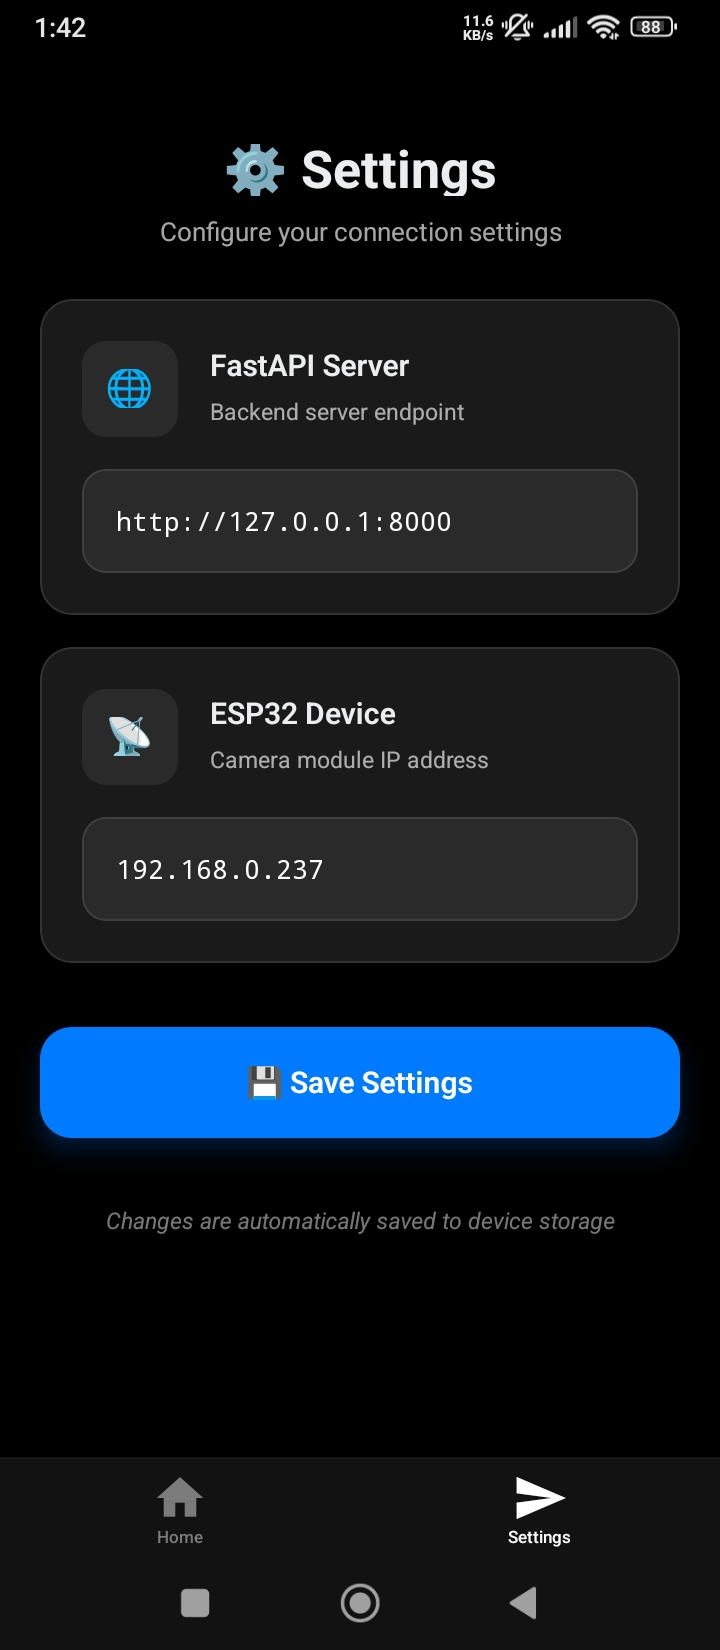
\includegraphics[width=.45\linewidth, keepaspectratio]{images/mobile_settings.jpg} % Ensure this is jpg
        \end{column}
    \end{columns}
    \vspace{0.5em}
    \footnotesize Key features shown: Connection status, capture controls (auto-capture interval, auto TTS), latest AI response display (on main screen, not fully visible here), configurable server/IP settings.
\end{frame}

\begin{frame}{Demonstration: Desktop Application}
    \framesubtitle{IntelliGaze - PyQt6 Desktop Client}
    \begin{figure}
        \centering
        \includegraphics[width=\textwidth, height=0.7\textheight, keepaspectratio]{images/desktop_main_ss.png}
        \caption{Desktop interface: Live ESP32-CAM feed, AI instruction input, AI response, and system logs.}
    \end{figure}
\end{frame}

% --- SECTION: Project Management ---
\section{Project Management}

\begin{frame}{Project Timeline: Gantt Chart}
    \framesubtitle{IntelliGaze Development Schedule (May 11 - June 10, 2025)}
    \begin{figure}
        \centering
        \includegraphics[width=\textwidth]{images/gantt_chart_image.png}
    \end{figure}
\end{frame}

% --- SECTION: Conclusion & Future ---
\section{Conclusion \& Future}

\begin{frame}{Conclusion}
    \framesubtitle{Summary of Achievements}
    \begin{figure}
        \centering
        \includegraphics[width=0.85\textwidth]{images/con.png}
    \end{figure}
\end{frame}

\begin{frame}{Future Works}
    \framesubtitle{Potential Enhancements for IntelliGaze}
    \begin{figure}
        \centering
        \includegraphics[width=0.85\textwidth]{images/kad.png}
    \end{figure}
\end{frame}

% --- SECTION: Team ---
\section{Team Contributions}
\begin{frame}{Team Contributions}
    \framesubtitle{Collaborative Efforts in IntelliGaze}
    \begin{itemize}
        \item \textbf{Touhidul Alam Seyam (230240003):}
            \begin{itemize}
                \item Project Lead \& Chief Architect; Overall system design, development, and end-to-end integration.
                \item Lead: React Native mobile app (UI/UX, logic, backend comms).
                \item Drove integration of all components; Key troubleshooting; Documentation lead.
            \end{itemize}
        \item \textbf{Shafiul Azam Mahin (230240022):}
            \begin{itemize}
                \item Lead: PyQt6 Desktop Application (GUI, video feed, direct AI service comms).
            \end{itemize}
        \item \textbf{Eftakar Uddin (230240004):}
            \begin{itemize}
                \item Lead: FastAPI Backend Server framework (API endpoints, server logic).
            \end{itemize}
        \item \textbf{Muntasir Rahman (230240002):}
            \begin{itemize}
                \item Lead: ESP32-CAM Firmware (camera init, WiFi, MJPEG streaming).
            \end{itemize}
        \item \textbf{Tasmim Akther Mim (230240025):}
            \begin{itemize}
                \item Lead: Text-to-Speech (TTS) functionality integration in mobile app (Groq API).
            \end{itemize}
    \end{itemize}
    \vspace{0.2em} % Reduced space
\end{frame}

% --- FINAL SLIDE ---
\begin{frame}{Thank You \& Q/A}
    \centering
    \Huge \textbf{Thank You!}
    \vspace{2em}

    \Large Questions?
    \vspace{3em}

    
\includegraphics[height=2cm]{images/logo.png}
    \hspace{1cm}
    
\includegraphics[height=2cm]{images/bgc-logo.png}
    
\end{frame}

\end{document}